%!TEX root = ../rapport.tex
%!TEX encoding = UTF-8 Unicode

% Chapitres "Introduction"

% modifié par Francis Valois, Université Laval
% 31/01/2011 - version 1.0 - Création du document

\chapter{Vision 2$^e$ itération}
\label{vision2}

\section{Localisation avec la caméra embarquée}

La localisation avec la caméra embarquée est un système de localisation d'appoint dans le projet Kinocto. La classe Localisation doit recevoir une image et une orientation grossière selon le nord, sud, est ou ouest par rapport à la table. Elle doit ensuite être initialisée en fournissant un fichier .xml contenant les paramètres de calibration. Ces paramètres comprennent les paramètres intrinsèques de la caméra obtenus lors de la calibration, les paramètres liés à la distorsion de l'image par la lentille, les paramètres extrinsèques qui permettent de lier les points des images prises par la caméra à leur position par rapport à un système de référence virtuel ainsi que les paramètres qui permettent de recadrer ces coordonnées par rapport au centre du robot.

Avec l'image et les paramètres provenant de la calibration, les méthodes de localisation, de détermination de l'orientation et de mesure de l'angle par rapport au mur peuvent être utilisées.

\subsection{Localisation}

\subsubsection{Transformations}

Pour effectuer la localisation du robot, il faut trouver dans l'image reçue au moins deux points identifiables dont les coordonnées par rapport à la table sont connues. Dans le projet Kinocto, ces points incluent les coins de la table, les coins inférieurs des blocs de couleur, les coins du carré vert dessiné sur la table. Pour passer du système de coordonnées du robot à celui de la table, il faut résoudre le système d'équations suivant, où les points $P_1A$ et $P2_A$ sont les points dans le système de la table, $P_1R$ et $P_2R$ sont les mêmes points dans le système du robot et $t_X$ et $t_Y$ sont les coordonnées du robot dans le système de la table:

\begin{equation}
\label{eq1}
X_{1A} = X_{1R}cos(\theta) - Y_{1R}sin(\theta) + t_X
\end{equation}
\begin{equation}
\label{eq2}
Y_{1A} = X_{1R}sin(\theta) + Y_{1R}cos(\theta) + t_Y
\end{equation}
\begin{equation}
\label{eq3}
X_{2A} = X_{2R}cos{\theta} - Y_{2R}sin(\theta) + t_X
\end{equation}
\begin{equation}
\label{eq4}
Y_{2A} = X_{2R}sin(\theta) + Y_{2R}cos(\theta) + t_Y
\end{equation}

En soustrayant l'équation~\ref{eq3} de l'équation~\ref{eq1} ainsi que l'équation~\ref{eq4} de l'équation~\ref{eq2}, on élimine $t_X$ et $t_Y$ et on se retrouve avec deux équations que l'on peut combiner pour obtenir une équation à une inconnue, $\theta$. Il s'agit d'une équation de la forme $a cos(\theta) + b sin(\theta) = c$. Ce type d'équation peut être résolu en considérant la relation suivante:

\begin{equation}
a cos(\theta) + b sin(\theta) = R cos(\theta - \alpha)
\end{equation}

Où $R = \sqrt{a^2 + b^2}$ et $tan(\alpha) = \frac{b}{a}$. En isolant $\theta$, on obtient donc:

\begin{equation}
\theta = cos^{-1}(\frac{c}{\sqrt{a^2 + b^2}}) + tan^{-1}(\frac{b}{a})
\end{equation} 

Il suffit ensuite d'utiliser $\theta$ dans deux des équations initiales pour retrouver les coordonnées du robot selon le système de référence de la table $t_X$ et $t_Y$.

\subsubsection{Localisation des points}

\begin{enumerate}
\item{Coins de table}

Les points correspondant aux coins de table sont trouvés dans l'image en effectuant d'abord une segmentation sur le noir et en utilisant ensuite l'algorithme des lignes de Hough pour retrouver les lignes de bas de mur. L'intersection entre les lignes de bas de mur constitue le coin de la table. Un intérêt de cette méthode est qu'elle permet de retrouver les coins de table même lorsqu'un obstacle se trouve devant celui-ci.

\item{Coins du bas des blocs de couleur}

Les coins du bas des blocs de couleurs peuvent être retrouvés en trouvant les intersections entre les lignes de bas de mur et la ligne du bas du bloc de couleur, trouvée après segmentation sur le bleu et l'orange.

\item{Coins du carré vert}

Les coins internes du carré vert peuvent être retrouvés en segmentant sur le vert et en retrouvant les intersections entre les lignes avec la méthode décrite plus haut.
\end{enumerate}

\subsection{Orientation et angle par rapport au mur}

L'angle par rapport au mur peut être utile pour réorienter le robot pour la lecture des sudokus. Il est facilement obtenu en utilisant la ligne de bas de mur détectée précédemment. L'orientation peut être déduite en utilisant cet angle et l'orientation fournie à l'initialisation.

\section{Orientation avec la caméra embarquée}

Après quelques essais avec la matrice de transformation, nous n'avons pas réussi à obtenir une localisation fiable avec la caméra embarquée. 

L'orientation avec la caméra embarquée a donc servi de méthode d'appoint à la localisation avec la Kinect pour corriger l'angle du robot à trois moments critiques, soit devant le mur lors de la lecture du sudocube, dans le carré vert avant le départ vers les sudocubes et dans le carré vert avant de commencer le dessin. 

L'angle est évalué en traçant des lignes de Hough sur des images segmentées sur le noir pour les murs et sur le vert pour le carré vert. La ligne pertinente est sélectionnée en trouvant la ligne croisant l'axe des y à la valeur la plus élevée et ayant la pente la plus faible. 

L'angle trouvé n'est pas l'angle réel du robot avec la ligne, mais un angle de 0° signifie que l'orientation du robot est correcte. L'erreur devient plus importante avec les grands angles, mais l'erreur d'orientation ne dépasse normalement pas 15°. En appliquant la correction 2 fois, l'orientation du robot est corrigée dans la plupart des cas.

\section{Extraire les contours d'un sudocube}

Au tout début, l'image est nettoyé de son bruit grâce a un flou gaussien.

La première étape d'extraction consiste à segmenter par couleur verte en convertissant l'image en HSV et en appliquant la méthode inRange() afin d'isoler le cadre vert du sudocube. Le contours du cadre est nettoyé avec l'application d'opérateur morphologique tel que la dilatation et l'érodation. Puis, les algorithmes d'opencv findContours() et approxPolyDP() sont appliqués pour trouver deux polygones rectangulaires. Ces polygones sont les bordures intérieures et extérieures du cadre. Enfin, on vérifie que l'aire des rectangles est plus grand que 200 000 pixels afin d'être sûr que ceux-ci sont assez grands pour être ceux du cadre du sudocube. Tous les polygones qui sont en bas de cette valeur sont soit des cadres vert des sudocubes adjacent qui n'occupent pas une grande partie de l'image ou des artéfacts dû à la segmentation qui ne nous intéressent pas.

\begin{figure}[h!]
\centering
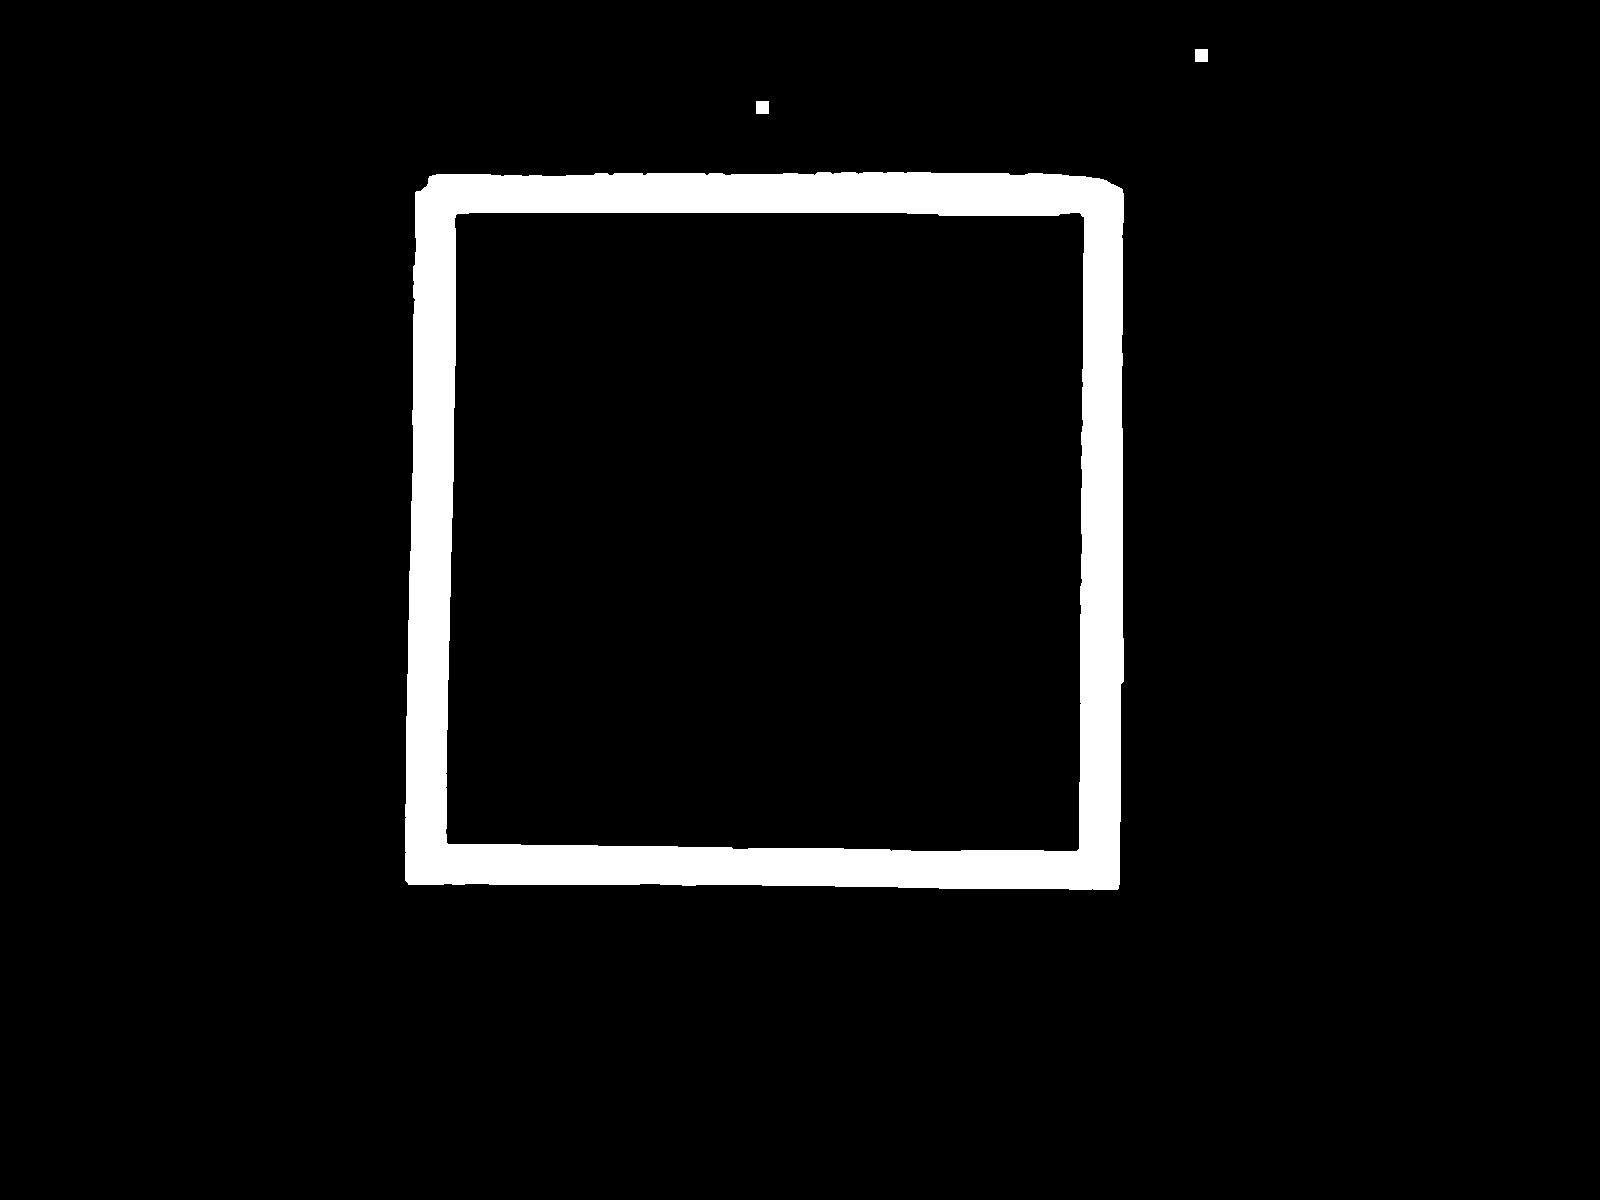
\includegraphics[scale=0.20]{fig/cadreVertSegmente.jpeg}
\caption{Exemple de segmentation sur le vert du cadre}
\label{fig:segmentation_vert}
\end{figure}

Ensuite, à partir du polygone intérieur du cadre on isole une sous-région de l'image principale que l'on recadre afin qu'elle ai 500 pixels de côté. L'image obtenue est convertie en noir et blanc avec la méthode threshold() pour appliquer le même algorithme de contour mentionné dans le premier paragraphe afin de trouver les polygones des cases du sudocube. Une dilatation et une érodation sont appliqué afin d'améliorer les contours des cases. Ensuite, on sélectionne tous les polygones qui ont une aire entre 150 et 700 pixels. Si jamais le nombre de polygones sélectionné n'est pas de 47, on réapplique la méthode threshold() avec un seuil de tolérance différent pour l'algorithme de contour et ce jusqu'à ce qu'on obtienne le bon seuil pour avoir 47 cases. 

Le polygone de la case rouge est obtenu en segmentant par couleur rouge et en appliquant à nouveau l'algorithme de contour mentionné ci-haut. 

\begin{figure}[h!]
\centering
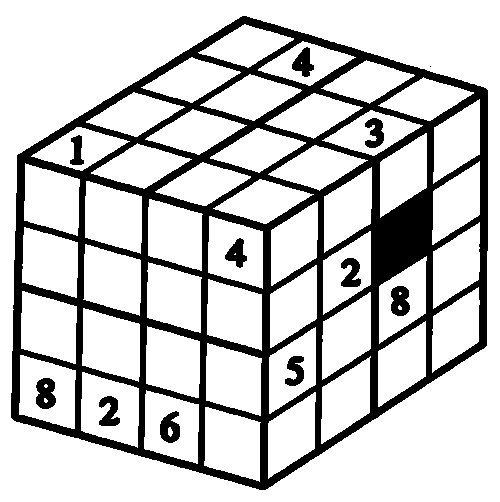
\includegraphics[scale=0.60]{fig/sudocubeThresh.jpeg}
\caption{Exemple de sudocube nettoyé et prêt à être extrait}
\label{fig:sudocube_thresh}
\end{figure}

Finalement, les images des cases sont triées en fonction de leur position en X et en Y dans l'image du sudocube et un algorithme de reconnaissance des caractères appliqué sur toutes les cases afin d'identifier les numéros. L'algorithme de reconnaissance utilise la technique KNearest. Les chiffres trouvés sont ajoutés dans la structure de données du sudocube et la position de la case rouge est spécifiée.

\begin{figure}[h!]
\centering

\includegraphics[scale=1]{fig/8Extrait.png}
\caption{Exemple de chiffre extrait}
\label{fig:chiffre_extrait}
\end{figure}

\subsection{Performance de l'algo}
L'algorithme prend en moyenne 250 ms afin de s'exécuter et réussi à extraire des sudocubes quand la caméra prend des photos entre 20 à 45 cm devant le mur avec un angle maximale de +-20 degrés de chaques côté. Sur 80 essais manuel un seul essais comportais un chiffre mal lu.

\section{Localisation avec la Kinect}

Pour aider au déplacement du robot, la Kinect a été utilisée afin de détecter la position des obstacles, la position du robot lui-même ainsi que sa position angulaire par rapport au point (0.0) de notre représentation cartésienne de la table. Toutefois, comme la Kinect est située à l'extérieur de la table de jeu, il faut une translation et une rotation des données obtenues afin de positionner les objets avec exactitude. Les 4 sections qui suivent expliquent en détail les différentes parties de l'algorithme de vision de la Kinect.

\subsection{Transformation des distances}
En premier lieu, il est important de clarifier quelles distances il est possible d'obtenir à l'aide de la Kinect. Le «Framework» OpenNI est capable de retourner 2 types de distances pour chacun des points dans l'image infrarouge obtenue de la Kinect. Le premier type de distances retourné est la longueur, en mètres, entre l'objectif et un point quelconque sur l'image. Le second type est dérivé du premier et correspond aux composantes X, Y et Z du vecteur de longueur entre l'objectif et la cible. Pour aider à la compréhension, les deux types de distances peuvent être représentés par les lignes vertes sur l'image \ref{fig:kinect_distance}. Toutefois, comme l'origine de notre représentation cartésienne de la table est située sur le coin inférieur droit de la table et que la Kinect n'est pas située à cet endroit, il est nécessaire d'obtenir la distance X et Y (lignes bleues sur l'image \ref{fig:kinect_distance}) entre l'origine et le point ciblé sur l'image obtenue de la Kinect. Pour y arriver, il suffit d'obtenir la position X et Y (lignes rouges sur l'image \ref{fig:kinect_distance}) de la lentille infrarouge de la Kinect ainsi que l'angle de la Kinect avec l'axe X de la table. Pour obtenir ces valeurs, nous utilisons une calibration simple présentée à la section \ref{s:kinectLocal}. Une fois la calibration effectuée, il est possible d'effectuer la transformation des distances de la Kinect vers les composantes X et Y recherchées à l'aide de règles de trigonométrie simples (Translation et Rotation). Toutefois, la Kinect possède une erreur de mesure qui augmente avec la distance. C'est pourquoi l'algorithme va toujours posséder une incertitude entre 1 et 3 cm pour chacun des points mesurés.

\begin{figure}[htbp]
\centering
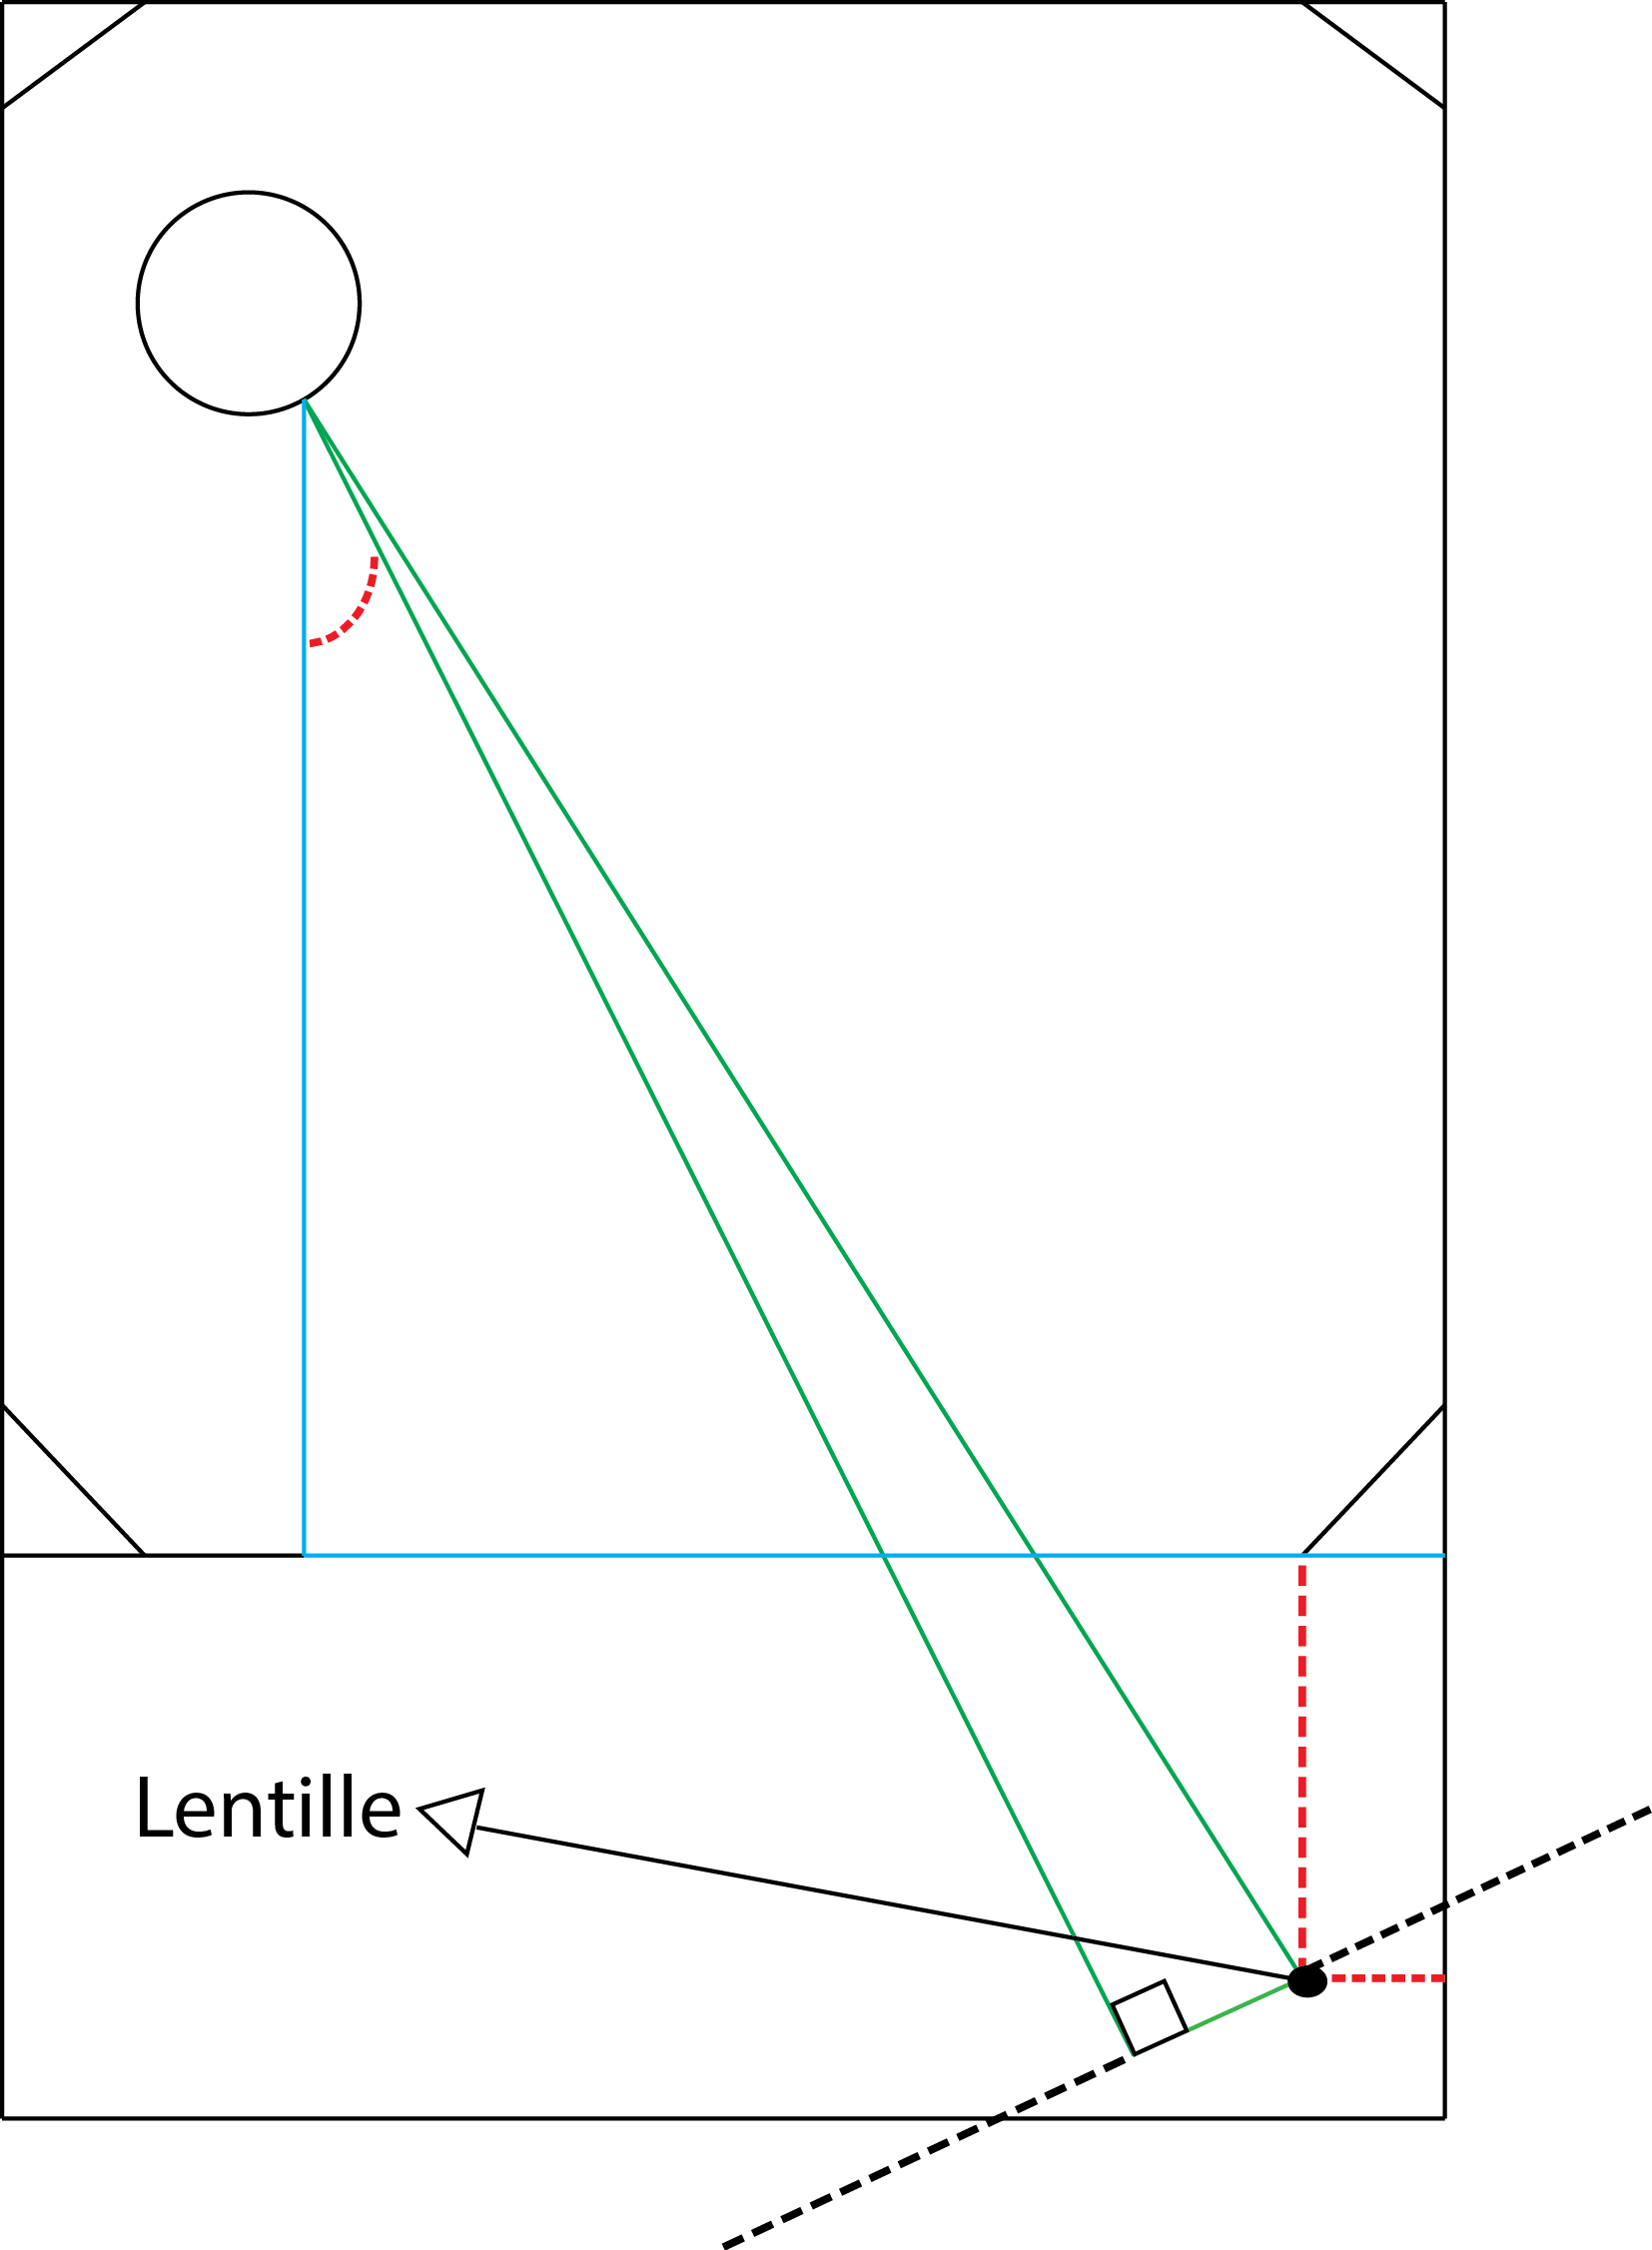
\includegraphics[scale=0.5]{fig/kinect_distance.png}
\caption{Schéma représentant la table et les différentes mesures obtenues avec la Kinect pour un point quelconque}
\label{fig:kinect_distance}
\end{figure}

\subsection{Localisation de la Kinect à l'aide de la calibration}
\label{s:kinectLocal}
Le but de la calibration est d'obtenir l'angle de la Kinect avec l'axe X de la table ainsi que la position de son objectif en XY par rapport au coin inférieur droit de la zone de jeu qui constitue notre point (0.0). Pour y arriver, un système, qui possède des dimensions connues, va positionner une plaque constituée d'un "Chessboard" sur la table à un endroit prédéterminé (ligne noire sur la table dans l'image \ref{fig:kinect_calibration}). Par la suite, une image RGB de la table est capturée à l'aide de la Kinect et les 2 points les plus éloignés horizontalement sur le "Chessboard" sont localisés. Ces 2 points sont reportés sur l'image de distances correspondante pour obtenir la distance XYZ de chacun des 2 points (lignes vertes sur l'image \ref{fig:kinect_calibration}). À l'aide de ces deux distances, les dimensions du petit triangle entre les deux points de la plaque de calibration sont trouvées (le triangle se situe en dessous de la plaque de calibration sur l'image \ref{fig:kinect_calibration}). En ayant les dimensions du triangle, il est possible de trouver l'angle de la Kinect, car celui-ci est le même que l'angle interne droit du triangle. Il suffit d'utiliser l'équation suivante avec les dimensions obtenues précédemment :

\begin{equation}
		Angle = \arctan \left( \frac{oppose}{adjacent} \right)
\end{equation}

\begin{figure}[htbp]
\centering
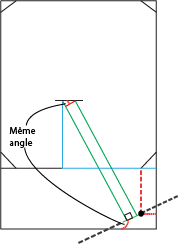
\includegraphics[scale=1]{fig/kinect_calibration.png}
\caption{Schéma représentant la table et les vecteurs nécessaires à la mesure de l'angle de la Kinect}
\label{fig:kinect_calibration}
\end{figure}

Pour obtenir la position de la Kinect, il est nécessaire de connaître la position réelle, par rapport au point (0.0), des 2 points utilisés pour la mesure de l'angle. En effectuant la rotation des distances de chacun, des points donnés par la Kinect pour ramener les mesures dans le plan XY de la table, les distances XY entre les points et l'objectif sont obtenus (lignes rouges pleines sur l'image \ref{fig:kinect_position}). En soustrayant les distances précédemment obtenues aux distances réelles mesurées (lignes bleues sur l'image \ref{fig:kinect_position}), la position de la Kinect est obtenue (lignes rouges pointillées sur l'image \ref{fig:kinect_position}).

\begin{figure}[htbp]
\centering
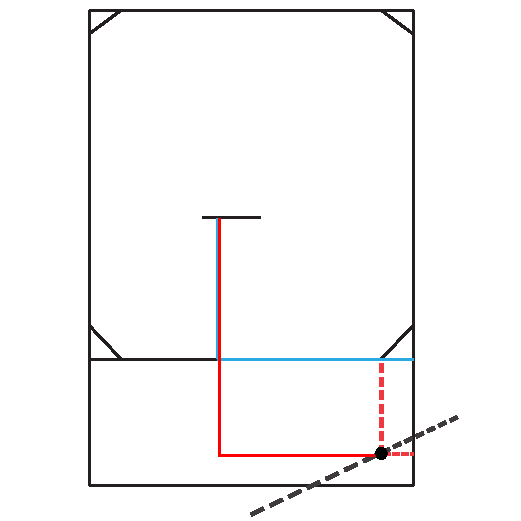
\includegraphics[scale=1]{fig/kinect_position.pdf}
\caption{Schéma représentant la table et les vecteurs nécessaires à la localisation de la Kinect}
\label{fig:kinect_position}
\end{figure}

\subsection {Réduction de la distorsion de la lentille infrarouge}
Dû à la distorsion présente dans la lentille de la caméra infrarouge de la Kinect, il a été nécessaire d'utiliser 2 algorithmes pour réduire la distorsion et améliorer la précision des distances obtenues.

\subsubsection{Correction à l'aide d'une transformation de perspective}
Le framework OpenCV possède une fonction de transformation de perspective qui se nomme "getPerspectiveTransform". Celle-ci reçoit en entrée une matrice de 4 points de distance selon un axe ainsi que les 4 mêmes points selon un autre axe. Par la suite, la fonction va produire une matrice de taille 3x3 pouvant être appliquée à n'importe quelle mesure qui doit passer d'un domaine à l'autre. Dans le cas du projet, le premier domaine est celui des distances retournées par la Kinect et le second est celui des distances réelles mesurées sur la table. Pour corriger la distorsion, il suffit alors de multiplier la matrice produite 3x3 par une matrice 3x1 composé des distances en x et z ainsi que du chiffre 1. Le résultat va être composé d'une mesure en x et z ainsi qu'un d'un facteur correctif devant être appliqué aux 2 mesures associées pour appliquer la correction. Ainsi, grâce à cette méthode, la précision augmente beaucoup en périphérie de l'image de points où la distorsion était très importante et pouvait causer des erreurs allant jusqu'à 8 centimètres.

\subsubsection{Correction à l'aide d'une courbe de correction d'erreur}
\label{s:distortion}
Le principal problème de la méthode précédente provient de son très petit nombre d'échantillons. Avec seulement 4 points, la distorsion ne peut être corrigée qu'aux alentours des points mesurés et il devient nécessaire de trouver une meilleure méthode pour corriger sur toute la plage de distances prévues. Comme la distorsion dépend de la distance avec l'axe optique, une courbe d'erreur de niveau 3 a été mise en place. Ainsi 16 différentes mesures situées un peu partout sur la table ont été effectuées à l'aide de la Kinect. Avec ces mesures, l'erreur de chacun des points avec la mesure réelle a été comptabilisée. Par la suite, une courbe d'interpolation a été créée pour relier les différents points d'erreurs et permettre une correction efficace de la distorsion en l'appliquant sur chacune des mesures effectuées.

\subsection{Détection des obstacles}
Comme il est possible d'obtenir n'importe quelle distance entre l'origine et un point quelconque sur l'image, un algorithme de recherche d'obstacles a été créé. Sachant que les obstacles sont situés dans une zone précise sur la table et que ceux-ci font 40cm de hauteur, il suffit de rechercher tout objet de cette hauteur situé dans la zone prédéfinie. La Kinect retourne la hauteur de chacun des points sur l'image infrarouge et permet de localiser les obstacles. De plus, à l'aide de calculs statistiques, l'algorithme est en mesure de trouver les obstacles lorsqu'ils sont presque alignés ou obstrués par un autre objet comme le robot. Comme cet algorithme dépend entièrement de l'algorithme de transformation des distances, les positions obtenues pour chacun des obstacles possèdent la même incertitude de 1 à 3 cm sur chaque mesure de distance effectuée. Pour améliorer la validité des mesures obtenues, une moyenne sur 3 images de distance est effectuée. En ce qui concerne l'efficacité de l'algorithme, différents tests montrent un temps de calcul d'environ 30 ms sur un Core 2 Duo 2.4 GHz pour obtenir la position du centre des deux obstacles.

\subsection{Détection du robot}
En ce qui concerne la détection du robot, un algorithme semblable à la détection des obstacles a été utilisé. Comme le robot possède une hauteur d'environs 20cm et une profondeur semblable, il est possible d'isoler, dans la matrice de distance, un carré qui correspond aux dimensions du robot. En plus de cette méthode, 2 "Chessboard" entourés d'un cadre bleu foncé sont placés sur 2 faces opposées du robot. En recherchant les carrés ainsi que les cadres bleues sur le robot, il est possible de déterminer sa position comme l'algorithme précédant, mais en plus d'obtenir son angle avec l'axe X de la table. Pour contrer l'erreur de position intrinsèque causée par la Kinect, la méthode de moyenne des distances utilisée pour la détection des obstacles est aussi appliquée à la détection du robot. Le temps de calcul est un peu plus élevé que la détection du robot et se situe aux alentours de 50 à 60 ms et il est possible d'obtenir une précision de moins de 2 centimètres dans le carré vert de la table. La précision à l'extérieur de celui-ci n'est pas nécessaire, car le robot se repositionne à l'aide de la Kinect seulement lors de la réception du signal Manchester et avant un dessin. 
